%%%%%%%%%%%%%%%%%%%%%%%%%%%%%%%%%%%%%%%%%%%%%%%%%%%%%%%%%%%%%%%%%%%%%%%%%%%%%%%%%%%%%%%%%%%
% Original author of template for CV (Plasmati Graduate CV v1.0 24/03/2013):
%  Alessandro Plasmati (alessandro.plasmati@gmail.com)
% Changes from the template onwards by (latest 30/01/2019):
% Pol del Aguila Pla (poldap@kth.se)
% Downloaded from:
%  http://www.LaTeXTemplates.com
% License:
%  CC BY-NC-SA 3.0 (http://creativecommons.org/licenses/by-nc-sa/3.0/)
% Important note (PdaP):
%  This template needs to be compiled with XeLaTeX.
%  The main document font is called Fontin and can be installed in sudo-enabled
%  Linux systems by running fixFONTproblem.sh (will internally call sudo when necessary).
%%%%%%%%%%%%%%%%%%%%%%%%%%%%%%%%%%%%%%%%%%%%%%%%%%%%%%%%%%%%%%%%%%%%%%%%%%%%%%%%%%%%%%%%%%

%----------------------------------------------------------------------------------------
%	PACKAGES AND OTHER DOCUMENT CONFIGURATIONS
%----------------------------------------------------------------------------------------

% Font and paper size
\documentclass[a4paper,10pt]{article}

% Font loading
\usepackage{fontspec} 
  \defaultfontfeatures{Mapping=tex-text}
  % Set main font for document
  \setmainfont[SmallCapsFont = Fontin SmallCaps]{Fontin} 

% Formatting
\usepackage{xunicode,xltxtra,url,parskip} 

% Coloring
\usepackage[usenames,dvipsnames]{xcolor} 

% Margin specification
\usepackage{fullpage}

% Links and other clickable references
\usepackage{hyperref} 
  % Link colors
  \definecolor{linkcolour}{rgb}{0,0.2,0.6}
  \hypersetup{colorlinks,breaklinks,urlcolor=linkcolour,linkcolor=linkcolour}

% Costumize section command
\usepackage{titlesec} % Used to customize the \section command
  % Text formatting
  \titleformat{\section}{\Large\scshape\raggedright}{}{0em}{}[\titlerule]
  % Spacing
  \titlespacing{\section}{0pt}{3pt}{3pt}

% Insert images
\usepackage{graphicx}

% Footnotes in tables
\usepackage{footnote}

% Tables that can span several pages
\usepackage{longtable}

% Several biblographies
\usepackage{bibunits}

% Trademark symbol
\usepackage{textcomp}

% Put references sections in the TOC (PDF and HTML links)
\usepackage[nottoc,numbib]{tocbibind}

\def\myname{P. del Aguila Pla}


\begin{document}

  % Remove page numbers
  \pagestyle{empty}

  %----------------------------------------------------------------------------------------
  %	NAME AND CONTACT INFORMATION
  %----------------------------------------------------------------------------------------

  \begin{center}
    \begin{tabular}{lcr}
	    \par{\centering{\Huge Pol \textsc{del Aguila Pla}}\bigskip\par} & & 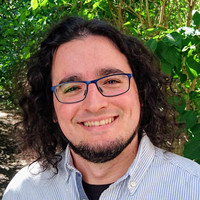
\includegraphics[width=0.3\textwidth]{../main/pol.jpg} \\
    \end{tabular}
  \end{center}
  
  \section{Personal data}
  
    \begin{tabular}{rl}
      \textsc{Place and date of birth:} & Barcelona, Catalonia, on 13 September 1990 \\
      \textsc{Home address:} & Carl Malmstens v\"{a}g 8, Lgh 1103, Solna, Sweden \\
      \textsc{Mobile phone:} & +46 (0)7-294-29302 \\
      \textsc{Email:} & \href{mailto:poldap@kth.se}{\nolinkurl{poldap@kth.se}} \\
      \textsc{Website:} & \href{https://poldap.github.io}{\nolinkurl{poldap.github.io}}
    \end{tabular}

  %----------------------------------------------------------------------------------------
  %  WORK EXPERIENCE 
  %----------------------------------------------------------------------------------------

  \section{Research experience}
  
    \begin{tabular}{r|p{13cm}}
    
      \textsc{2019 Sept} 	& Ph.D. Thesis \\
      \textsc{2014 Sept} 	& \emph{Inverse problems in signal processing: Functional optimization, parameter estimation and machine learning} \\
				& \footnotesize{ Division of Information Science and Engineering, School of Electrical Engineering and Computer Science,
				  \textbf{KTH} Royal Institute of Technology, Stockholm, Sweden. Supervisor: \textbf{Prof. Joakim Jald\'{e}n}. 
				  Opponent: \textbf{Prof. Yonina Eldar}, Weizmann Institute of Science, Israel.
				  Defense date: 16 Sept 2019.
				  } \\
      \multicolumn{2}{c}{} \\

      \textsc{2014 Sept} 	& Research Engineer \\
      \textsc{2014 Mar} 	& \emph{Probability density estimation, a review of the state of the art.} \\ 
				& \footnotesize{Department of Signal Processing, School of Electrical Engineering,
				  \textbf{KTH} Royal Institute of Technology, Stockholm, Sweden. Supervisor: \textbf{Prof. Joakim Jald\'{e}n}.} \\
      \multicolumn{2}{c}{} \\
      %------------------------------------------------

      \textsc{2014 Mar} 	& Master's thesis \\
      \textsc{2013 Aug} 	& \emph{ Normalization of remote sensing imagery for automatic information extraction } \\ 
				& \footnotesize{Department of Communication Theory, School of Electrical Engineering,
				  \textbf{KTH} Royal Institute of Technology, Stockholm, Sweden. Supervisors and examiner: \textbf{Dr. Felipe Calderero, Prof. Ferran Marqu\'{e}s and Prof. Markus Flierl}.} \\
      \multicolumn{2}{c}{} \\

      %------------------------------------------------

      \textsc{2012 Aug} 	& Undergraduate research \\
      \textsc{2012 Apr} 	& \emph{Image analysis for sport events classification, a review of the state of the art.} \\ 
				& \footnotesize{Image Processing Group (GPI), Department of Signal Theory and 
				  Communications (TSC), \emph{Escola T\`{e}cnica Superior d'Enginyeria de Telecomunicaci\'{o} 
				  de Barcelona}, \textbf{UPC BarcelonaTech}. Supervisor: \textbf{Prof. Ferran Marqu\'{e}s}.} \\

    \end{tabular}

  %----------------------------------------------------------------------------------------
  %	EDUCATION
  %----------------------------------------------------------------------------------------

  \section{University education}

    \begin{tabular}{r|p{13cm}}	
    
      \textsc{2014 Mar}  & \emph{Civilingenj\"{o}r}, 5-year degree in \textbf{Electrical Engineering} \\
      \textsc{2012 Aug}  & \footnotesize{\textbf{KTH Royal Institute of Technology}, School of Electrical Engineering, Stockholm, Sweden. 
			   Heavily specialized in signal processing and its applications to communications and imaging. Double degree program.} \\ 
      \multicolumn{2}{c}{} \\

      %------------------------------------------------
      
      \textsc{2014 Mar}  & \emph{Enginyer de Telecomunicaci\'{o}}, 5-year degree in \textbf{Telecommunications Engineering} \\  
      \textsc{2008 Sep}  & \footnotesize{\textbf{UPC BarcelonaTech}, \emph{Escola T\`{e}cnica Superior
			   d'Enginyeria de Telecomunicaci\'{o} de Barcelona}, Barcelona, Catalonia. 
			   Specialized in signal processing and its applications to pattern recognition and speech processing. Double degree program.} \\
    \end{tabular}

  %----------------------------------------------------------------------------------------
  %	PUBLICATIONS
  %----------------------------------------------------------------------------------------
  \begin{bibunit}[IEEEtran_Pol]
    \renewcommand\refname{Publications}
    \nocite{AguilaPla2019b,AguilaPla2019a,AguilaPla2019,AguilaPla2017,AguilaPla2017a,AguilaPla2018,AguilaPla2018a,AguilaPla2014}
    \footnotesize{
    \putbib[../pubs/bibfile]}
   
    \section{Impact case - Patent and product}
        
        The technology developed in \cite{AguilaPla2017,AguilaPla2017a}, protected by \cite{Mabtech2017},
        was implemented by Mabtech AB and Quamcom Research \& Technology AB, resulting on a successful product
        for biomedical researchers by the name of Mabtech IRIS (\url{https://www.mabtech.com/iris}).
        %The comercialization and further development of this product currently involves $4$ full-time jobs at Mabtech AB. 
        References at Mabtech AB: \textbf{Dr.~Christian~Smedman} and \textbf{Prof.~Staffan~Paulie}.
    
  \end{bibunit}
  
  %----------------------------------------------------------------------------------------
  %	SCHOLARSHIPS AND ADDITIONAL INFO
  %----------------------------------------------------------------------------------------
  \section{Grants and awards}
    \begin{savenotes}
    \begin{tabular}{r|p{13cm}}
      % Gålöstiftelsen 14000 SEK
      % EECS Malme stiftelsen 21200 SEK
      % Wallenberg jubilee 4700 SEK
      % KTH Opportunities 13200 SEK
      % KVA Engineering sciences 19038 SEK
      % Åforsk 6000 SEK
      % Current sum: 78138 SEK
      \textsc{2019 Mar} & Travel grants. Total amount $\approx 78\,\mathrm{kSEK}\approx 8.4\,\mathrm{k\$} $.\\
      \textsc{2017 Sep} & \footnotesize{Gålöstiftelsen study \textbf{travel grant},
              Malme's foundation \textbf{travel grant} through the EECS school at KTH, 
              KTH Opportunities Fund \textbf{project scholarship},
			  Knut and Alice Wallenberg Jubilee appropriation \textbf{travel grant},
			  \AA forsk Foundation \textbf{travel grant}, and 
			  Engineering Sciences 2017 call from The Royal Swedish
			  Academy of Sciences (KVA, call ES2017-0011) \textbf{project and travel 
			  grant.}} \\
      \multicolumn{2}{c}{} \\
      
      \textsc{2013 Mar} & Exchange studies scholarships \\ 
      \textsc{2012 Aug} & \footnotesize{\textbf{Erasmus} and \textbf{AGAUR}\footnote{~Catalan Agency for Management of University and Research Grants} exchange studies scholarships.}  \\
      \multicolumn{2}{c}{} \\

      \textsc{2009 Jun}	& Promotion's top-10 award. Ranked $4^{\mathrm{th}}$. \\
      \textsc{2008 Sep}	& \footnotesize{Receiver of the UPC BarcelonaTech award for \textbf{first 
			  year students with top-10 grades} in Telecommunications Engineering.} \\

    \end{tabular}
    \end{savenotes}

  %----------------------------------------------------------------------------------------
  %	Contact with the scientific community
  %----------------------------------------------------------------------------------------
  
  \section{Participation in the scientific community}
    
    \begin{longtable}[H]{r|p{13.5cm}}
      
      \emph{Current}	& Reviewer for \textbf{Elsevier Signal Processing} \\
      \textsc{2019 Mar} &  \\
      \multicolumn{2}{c}{} \\
      
      \emph{Current}	& Reviewer for the \textbf{IEEE Transactions on Signal Processing} \\
      \textsc{2015 Aug} &  \\
      \multicolumn{2}{c}{} \\
      
      
      \textsc{2019 Apr} &  \textsc{12-13 Apr}, Invited participant in the 2019 IEEE Signal Processing Society (SPS) Long Range Planning Meeting\\
      & \\
      & Lecture presentation (\textsc{9 Apr}) within the \emph{2019 IEEE $16^{\mathrm{th}}$ International
			  Symposium on Biomedical Imaging} (\textbf{ISBI 2019}), titled 
			  \textbf{SpotNet --- Learned iterations for cell detection in image-based immunoassays}, access at \href{https://embs.papercept.net/conferences/scripts/myprogram.pl?ConfID=79&Add=208}{\texttt{embs.papercept.net}}.\\
			  & \footnotesize{Hilton Molino Stucky, Venice, Italy.} \\  
			  \multicolumn{2}{c}{} \\
			  
			  
    
      \textsc{2019 Jan} & \textsc{7 Jan - 7 Feb}, Research visit at \textbf{Professor Jean-Luc Starck}'s group (\textbf{CosmoStat}). \\
                        & \footnotesize{Department of Astrophysics, \textbf{CEA Paris-Saclay}, Paris, France} \\
                        & \\
                        & \textsc{14 and 28 Jan}, presentations at \textbf{Cosmostat} and \textbf{Parietal}, \textbf{NeuroSpin}, \textbf{INRIA}, respectively, titled \emph{Cell detection by functional inverse diffusion and non-negative group sparsity - Biology, physics, math and engineering}, access at \href{http://www.cosmostat.org/events/cosmoclub/cosmosclub-pol}{\texttt{www.cosmostat.org}} and \href{https://team.inria.fr/parietal/slides-of-pol-del-aguila-plas-talk-available-now-online/}{\texttt{team.inria.fr/parietal}}. \\
      \multicolumn{2}{c}{} \\
    
      \textsc{2018 Jul} & Attendance to the \emph{Thirty-fifth International Conference on Machine
						  Learning} (\textbf{ICML 2018}). \\
						& \footnotesize{Stockholmsm\"{a}ssan, Stockholm, Sweden.} \\
	  \multicolumn{2}{c}{} \\
						
      \textsc{2018 Jun} & Poster presentation within the \emph{SIAM Conference on Imaging Science}
			  (\textbf{SIAM-IS 2018}), titled \textbf{Source localization by spatially
			  variant blind deconvolution}, access at \href{https://www.siam-is18.dm.unibo.it/uploads/store/a7a8b242b168225d0be8998fa373f58b.pdf}{\texttt{www.siam-is18.dm.unibo.it}}. \\
			& \footnotesize{\textbf{University of Bologna}, Bologna, Italy.}\\
      \multicolumn{2}{c}{} \\
    
      \textsc{2018 Apr} & Poster presentation within the \emph{IEEE International Conference 
			  on Acoustics, Speech and Signal Processing} (\textbf{ICASSP 2018}), titled
			  \textbf{Convolutional group-sparse coding and source localization}, access at \href{https://sigport.org/documents/convolutional-group-sparse-coding-and-source-localization}{\texttt{sigport.org}}. \\
			& \footnotesize{Calgary Talus Convention Centre, Calgary, Alberta, Canada.} \\
			& \\
			& \textsc{9 - 13 Apr}, Research visit at \textbf{Professor Stephen P. Boyd's group}. \\
			& \textsc{10 Apr}, Presentation to the group titled 
              \emph{Cell detection by functional inverse diffusion and non-negative group sparsity}.\\
			& \footnotesize{Information Systems Laboratory, Department of \textbf{Electrical Engineering, 
			  Stanford University}, Stanford, California, United States of America} \\
			& \\
			& Poster presentation within the \emph{2018 IEEE $15^{\mathrm{th}}$ International
			  Symposium on Biomedical Imaging} (\textbf{ISBI 2018}), titled
			  \textbf{Cell detection on image-based immunoassays}.\\
			& \footnotesize{Omni Shoreham Hotel, Washington, D.C., United States of America.} \\
      \multicolumn{2}{c}{} \\
      
      \textsc{2017 Nov} & Lecture presentation within the workshop \emph{Generative models, 
			  parameter learning, and sparsity} (VMVW02), titled
			  \textbf{Cell detection by functional inverse diffusion and group sparsity},
			  access at \href{https://downloads.sms.cam.ac.uk/2600830/2600858.mp4}{\texttt{downloads.sms.cam.ac.uk}}. \\
			& \footnotesize{\textbf{Isaac Newton Institute for Mathematical Sciences},
			  \textbf{University of Cambridge}, Cambridge, United Kingdom.
			  Within the programme \emph{Variational methods and effective
			  algorithms for imaging and vision}.}\\

    \end{longtable}
  
  %----------------------------------------------------------------------------------------
  %	TEACHING EXPERIENCE
  %----------------------------------------------------------------------------------------
  \section{Teaching experience}
  
    \begin{bibunit}[IEEEtran_Pol]
    \begin{tabular}{r|p{13cm}}
      
      \emph{Current}	 & Supervision of Master's and Bachelor's thesis (see below) \\
      \textsc{2017 Feb}  & \footnotesize{Main supervisor of two master's thesis, \cite{Jones2018} and one
                            ongoing. 
							Designer of two bachelor's thesis projects, attracting $5$ 
							different groups of two students. Main supervision for $2$ bachelor's 
							thesis \cite{F2A2018,F2B2018}, and co-supervisor for six,
							\cite{F3A2018,F3B2018,F3C2018} and three ongoing. } \\      
      \multicolumn{2}{c}{} \\
      
	  \textsc{2018 Dec}     & Teaching assistance in the course \textbf{EQ2300: Digital Signal Processing} \\
	  \textsc{2014 Sep} & \footnotesize{Taught every year \textsc{Nov -- Dec} by Prof. Joakim Jald\'{e}n and 
							one to three assistants. Approximate numbers: $120\,\mathrm{h}$ of guidance of 
							exercise sessions and lectures, $140\,\mathrm{h}$ of 
							class preparation, $45\,\mathrm{h}$ of course and material development,
							$100\,\mathrm{h}$ of grading of projects and exams, and $20\,\mathrm{h}$ of private tutoring.} \\
     
    \end{tabular}

	
      \renewcommand\refname{\normalsize{Supervised theses}}
	  \footnotesize{
      \putbib[../pubs/bibfile_students]}
	\end{bibunit}
  
  %----------------------------------------------------------------------------------------
  %	LANGUAGES
  %----------------------------------------------------------------------------------------

  \vspace{-10pt}
  
  \section{Languages}

    \begin{tabular}{rp{10cm}}
      
      \textsc{Mother tongue (C2+):} & Catalan and Spanish \\
      
      \textsc{Professional (C2):} & English \\
      
      \textsc{Conversational (B2):} & Swedish \\
      
      \textsc{Basic (A1-A2):} & Italian and French (\textsc{DELF} A2, \textsc{2006 Aug})
      
    \end{tabular}

  %----------------------------------------------------------------------------------------
  %	COMPUTER SKILLS 
  %----------------------------------------------------------------------------------------

  \vspace{-15pt}
  
  \section{Other skills}

  \begin{tabular}{rp{12cm}}
	Technical skills:  & Experienced in the administration of GPU-enabled Linux computational servers.
						 Experienced in the maintenance of websites for academic groups.
						 Professional in electronic design and measurement, network testing and 
						 simulation, measurement of digital communications systems, and antenna design
						 and performance analysis. \vspace{5pt}\\ 
	Programming:       &  \textsc{C/C++, Java, R, Python, TensorFlow, Bash, Matlab, \LaTeX}  \vspace{5pt}\\ 
	Soft skills: 	   & Social and friendly collaborator. Accomplished and praised supervisor of 
						 student theses and teacher of exercise sessions. Very attentive to 
						 detail. Experienced in academia--industry collaborations.

  \end{tabular}

  %----------------------------------------------------------------------------------------
  % INTERESTS AND ACTIVITIES
  %----------------------------------------------------------------------------------------

  \vspace{-15pt}
  
  \section{Interests and activities}

    Linux, Free / Libre / Open-source software. Open-access research and open science. Philosophy and sociology. \\
    Regular opera-goer, moderate cinephile, initiated tap-dancer and avid reader. \\
    Hiking enthusiast and ex-capoeira practicioner.

\end{document}
